\documentclass[mathserif]{beamer}
\usepackage[utf8]{inputenc}
\usepackage[T1]{fontenc}
\usepackage{array}
\usepackage{amsmath,amssymb,latexsym,epic,eepic,epsfig,graphics,psfrag}
\usepackage{amsfonts,amsbsy}
\usepackage{subfigure}
\definecolor{mygray}{RGB}{244,244,244}
\usepackage[scaled]{beramono}
\usepackage{listings}
\lstset {                 % A rudimentary config that shows off some features.
    language=R,
    basicstyle=\scriptsize\ttfamily, % Without beramono, we'd get cmtt, the teletype font.
    commentstyle=\textit, % cmtt doesn't do italics. It might do slanted text though.
    keywordstyle=,
    identifierstyle=,
    aboveskip=12pt,
    abovecaptionskip=6pt,
    framextopmargin=4pt,
    framexbottommargin=4pt,
    framexleftmargin=4pt,
    framexrightmargin=4pt,
    xleftmargin=4pt,
    xrightmargin=4pt,
    backgroundcolor=\color{mygray},
    frame=single,
    showstringspaces=false,
    captionpos=b,
    tabsize=4            % Or whatever you use in your editor, I suppose.
}
\newcommand\myvec[1]{\boldsymbol{#1}}
\newcommand\myverb[1]{{\footnotesize\texttt{#1}}}
\newcommand\Corr[1]{\textrm{Corr}[#1]}
\newcommand\given{\,|\,}
\newcommand\respath[1]{../results/#1}
\usefonttheme{structurebold}
\usetheme{Copenhagen}
\author{Anders Hørsted -- s082382}
\institute{02433 Hidden Markov Models}
\date{May 31th 2012}


\title[Presentation of exercise 1]{Presentation of written exercise 1}
\begin{document}

\begin{frame}
\titlepage
\end{frame}


\begin{frame}{Quick remarks}
    \begin{itemize}
    \item I forgot to put a hat on the parameter estimates. The estimate of $\myvec{\Gamma}$ should have been denoted $\widehat{\myvec{\Gamma}}$ etc.
    \end{itemize}
\end{frame}


\begin{frame}{Dataset for the exercise}
\begin{figure}[ht]
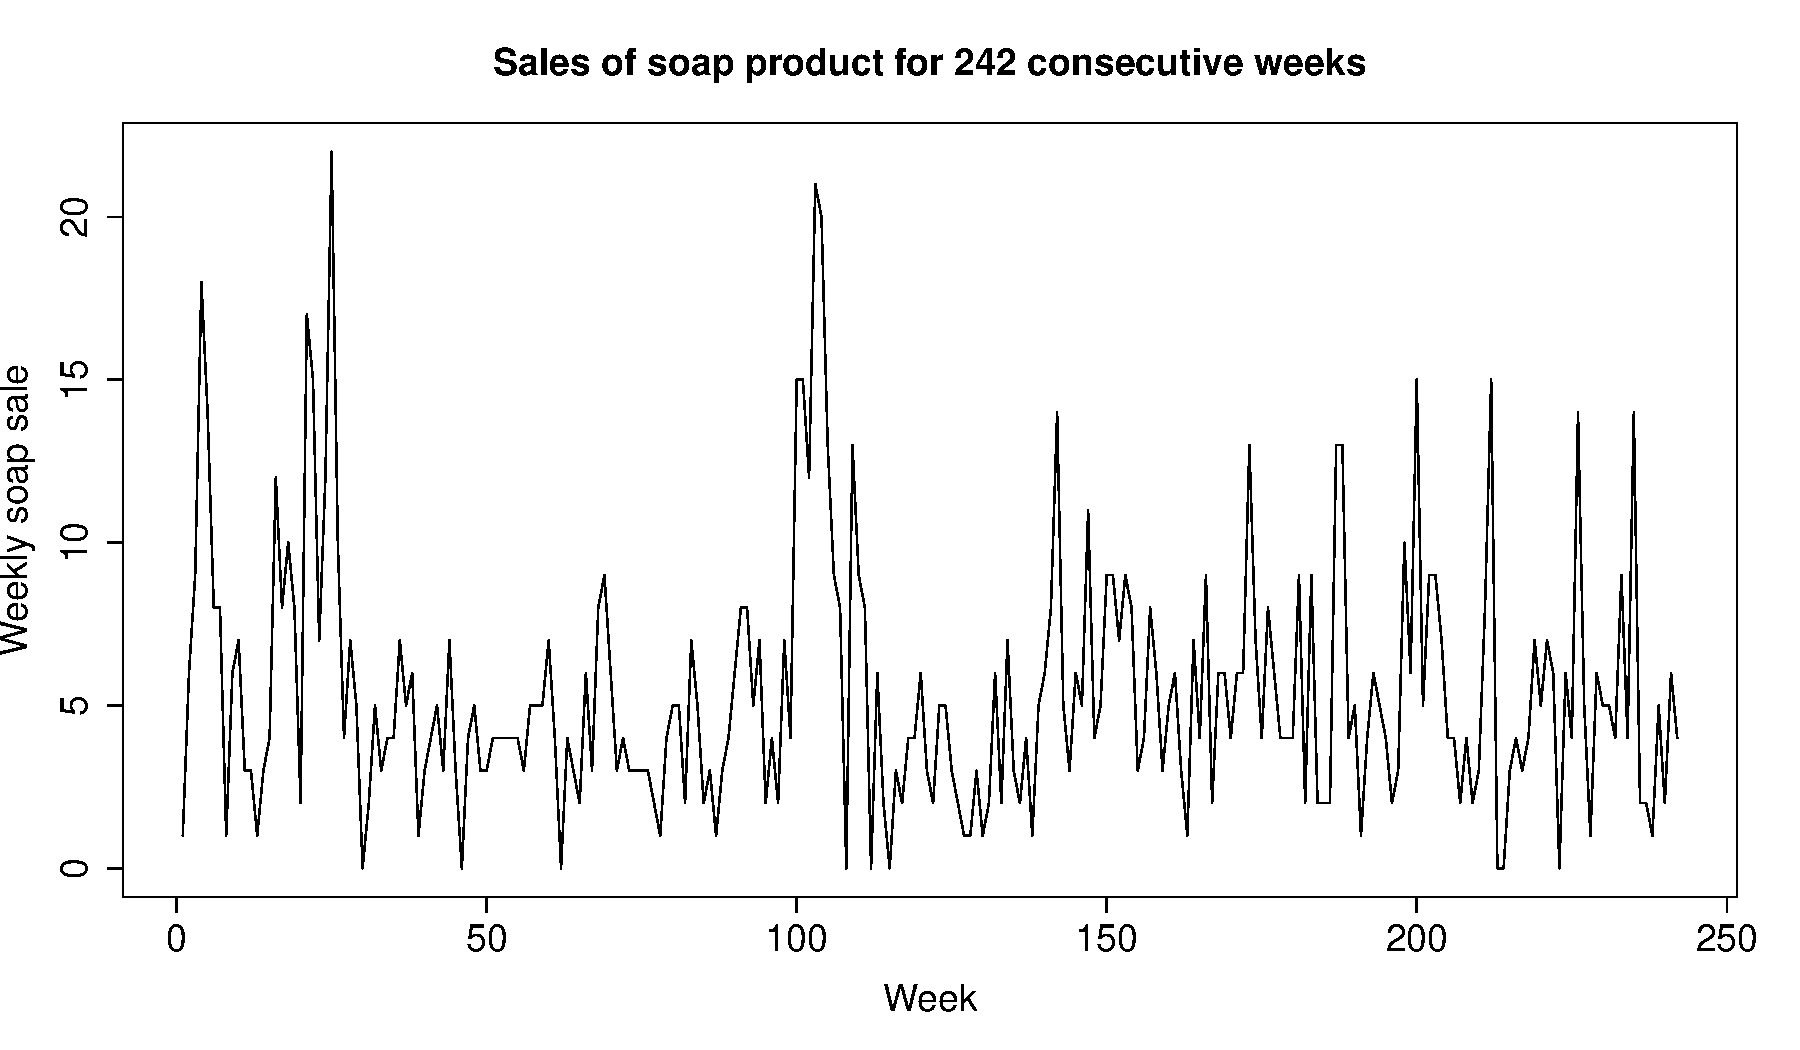
\includegraphics[width=260px]{../plots/sales-series.pdf}
\end{figure}
\vspace{-0.5cm}
Count data so Poisson seems natural. But $\bar{x}=5.44$ and $s^2=15.40$, so the data is overdispersed. Also the data is serially correlated so a simple Poisson mixture will not work. HMM to the rescue.
\end{frame}

\begin{frame}{Poisson HMM}
    2-, 3- and 4-state Poisson HMM was fitted to the data.
    \begin{table}[ht]
        \tiny
        \centering
        \begin{tabular}{cccccccccccc}
            \hline
             & $\mu$ & $\sigma^2$ & $\rho_1$ & $\rho_2$ & $\rho_3$ & $\rho_4$ & $\rho_5$ & $\rho_6$ & $\rho_7$ \\\hline
            Sample & 5.442 & 15.401 & 0.392 & 0.250 & 0.178 & 0.136 & 0.038 & 0.044 & 0.052 \\
2-states & 5.429 & 13.784 & 0.329 & 0.178 & 0.097 & 0.052 & 0.028 & 0.015 & 0.008 \\
3-states & 5.421 & 14.721 & 0.407 & 0.268 & 0.178 & 0.120 & 0.081 & 0.055 & 0.037 \\
4-states & 5.418 & 14.779 & 0.380 & 0.241 & 0.157 & 0.103 & 0.067 & 0.044 & 0.029 \\
        \end{tabular}
    \end{table}
    \begin{table}[ht]
        \tiny
        \centering
        \begin{tabular}{ccc}
            \hline
             & AIC & BIC \\\hline
            2-states & 1245.337 & 1259.292 \\
3-states & 1239.043 & 1270.444 \\
4-states & 1240.528 & 1296.351 \\
        \end{tabular}
    \end{table}
    The 3-state model has the best AIC and the 2-state model has the best BIC. Better correspondance between the sample correlations and the correlations for the 3-state model makes the 3-state model the winner.
\end{frame}

\begin{frame}{The 3-state model}
    \begin{figure}
    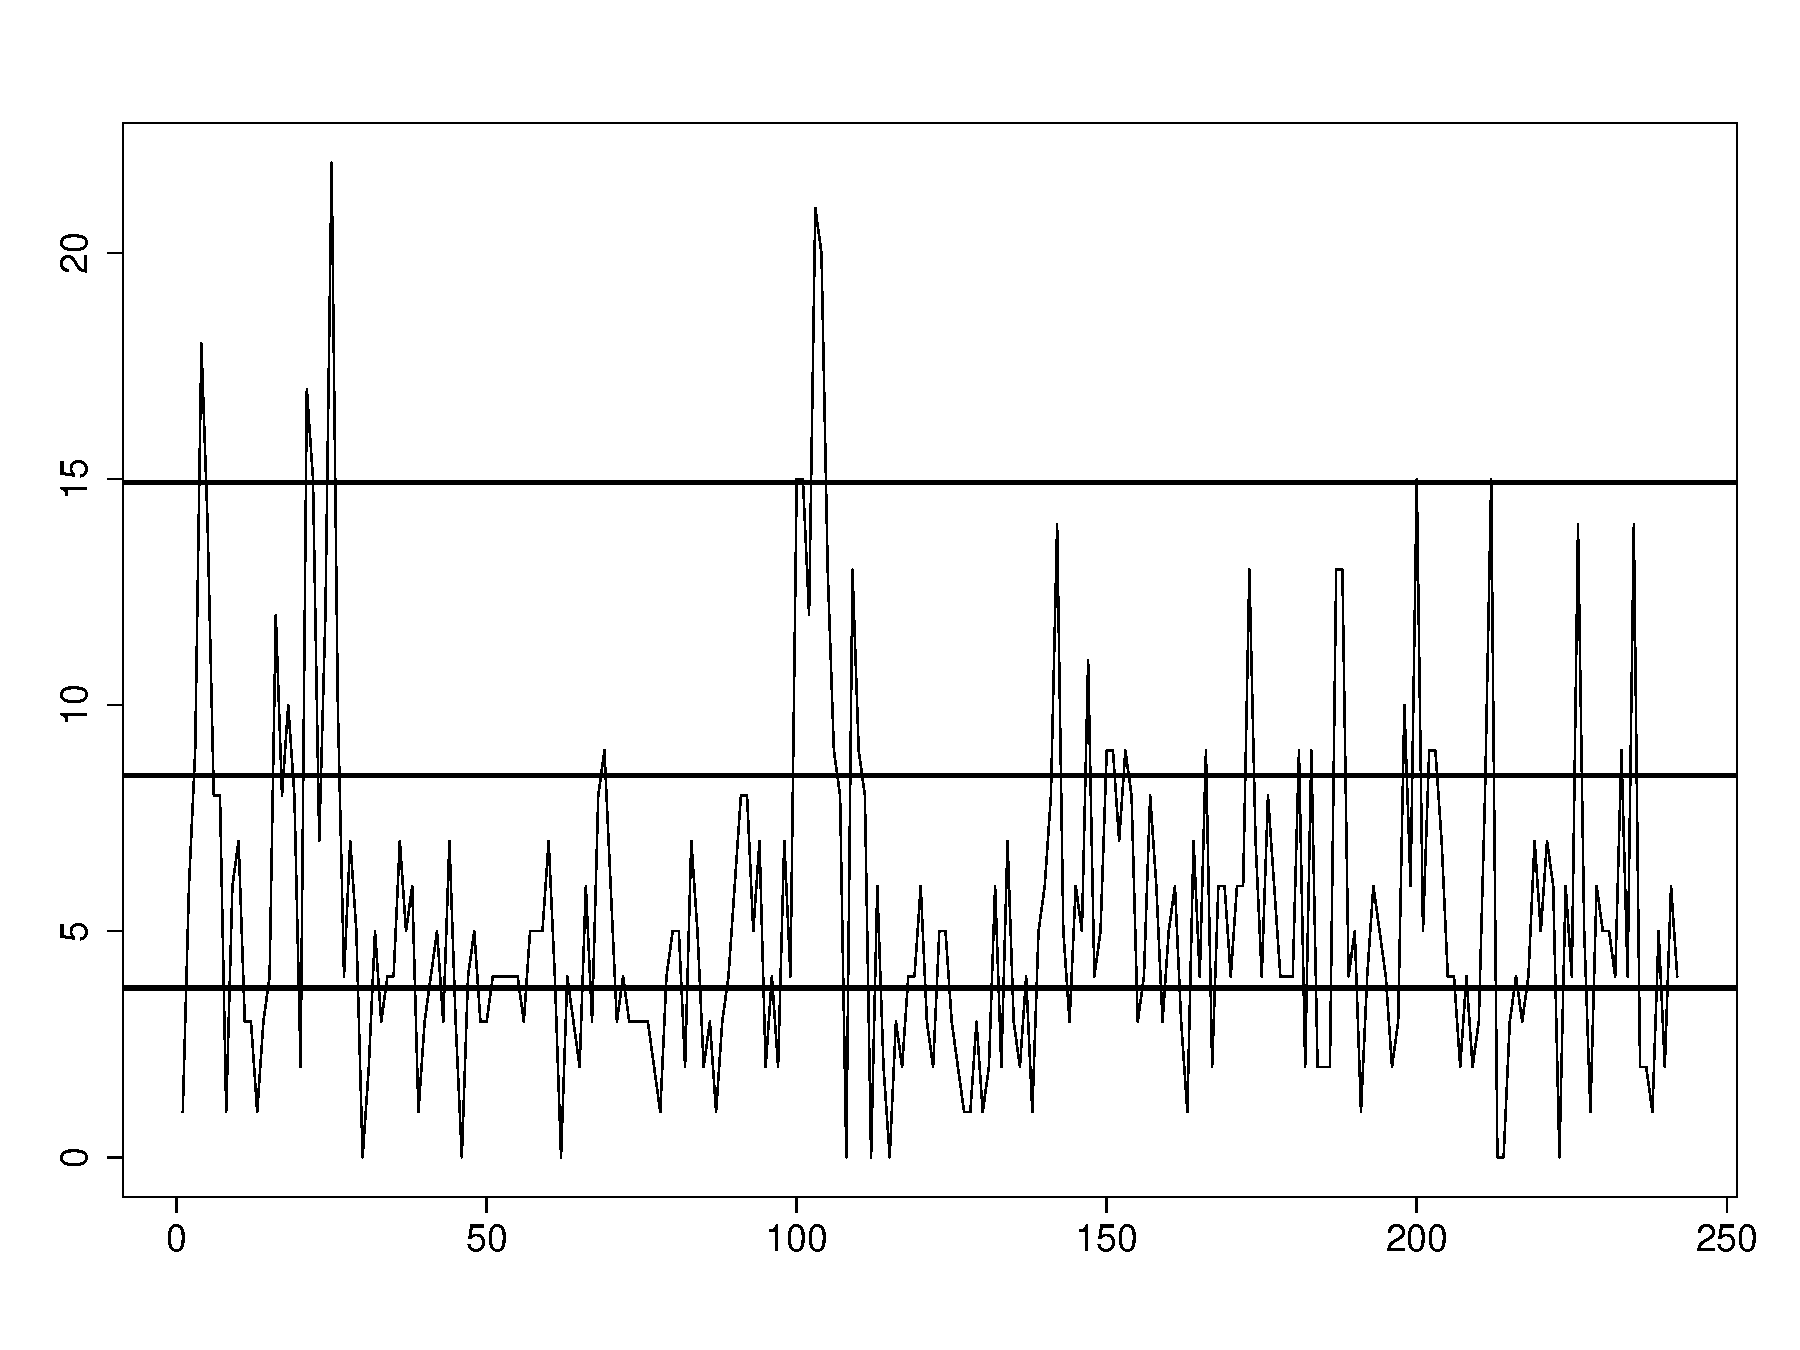
\includegraphics[width=180px]{../plots/3-state-ml-means-on-data.pdf}
    \end{figure}
    \begin{equation*}
        \myvec{\Gamma} = \input{\respath{3-state-ml-gamma.tex}} \quad\quad
        \myvec{\lambda} = \input{\respath{3-state-ml-lambda.tex}} 
    \end{equation*}
    \begin{equation*}
        \myvec{\delta} = \input{\respath{3-state-ml-delta.tex}}
    \end{equation*}
    {\it and still no hats on the parameter estimates}
\end{frame}

\begin{frame}{Model check}
    \begin{figure}
    \only<1>{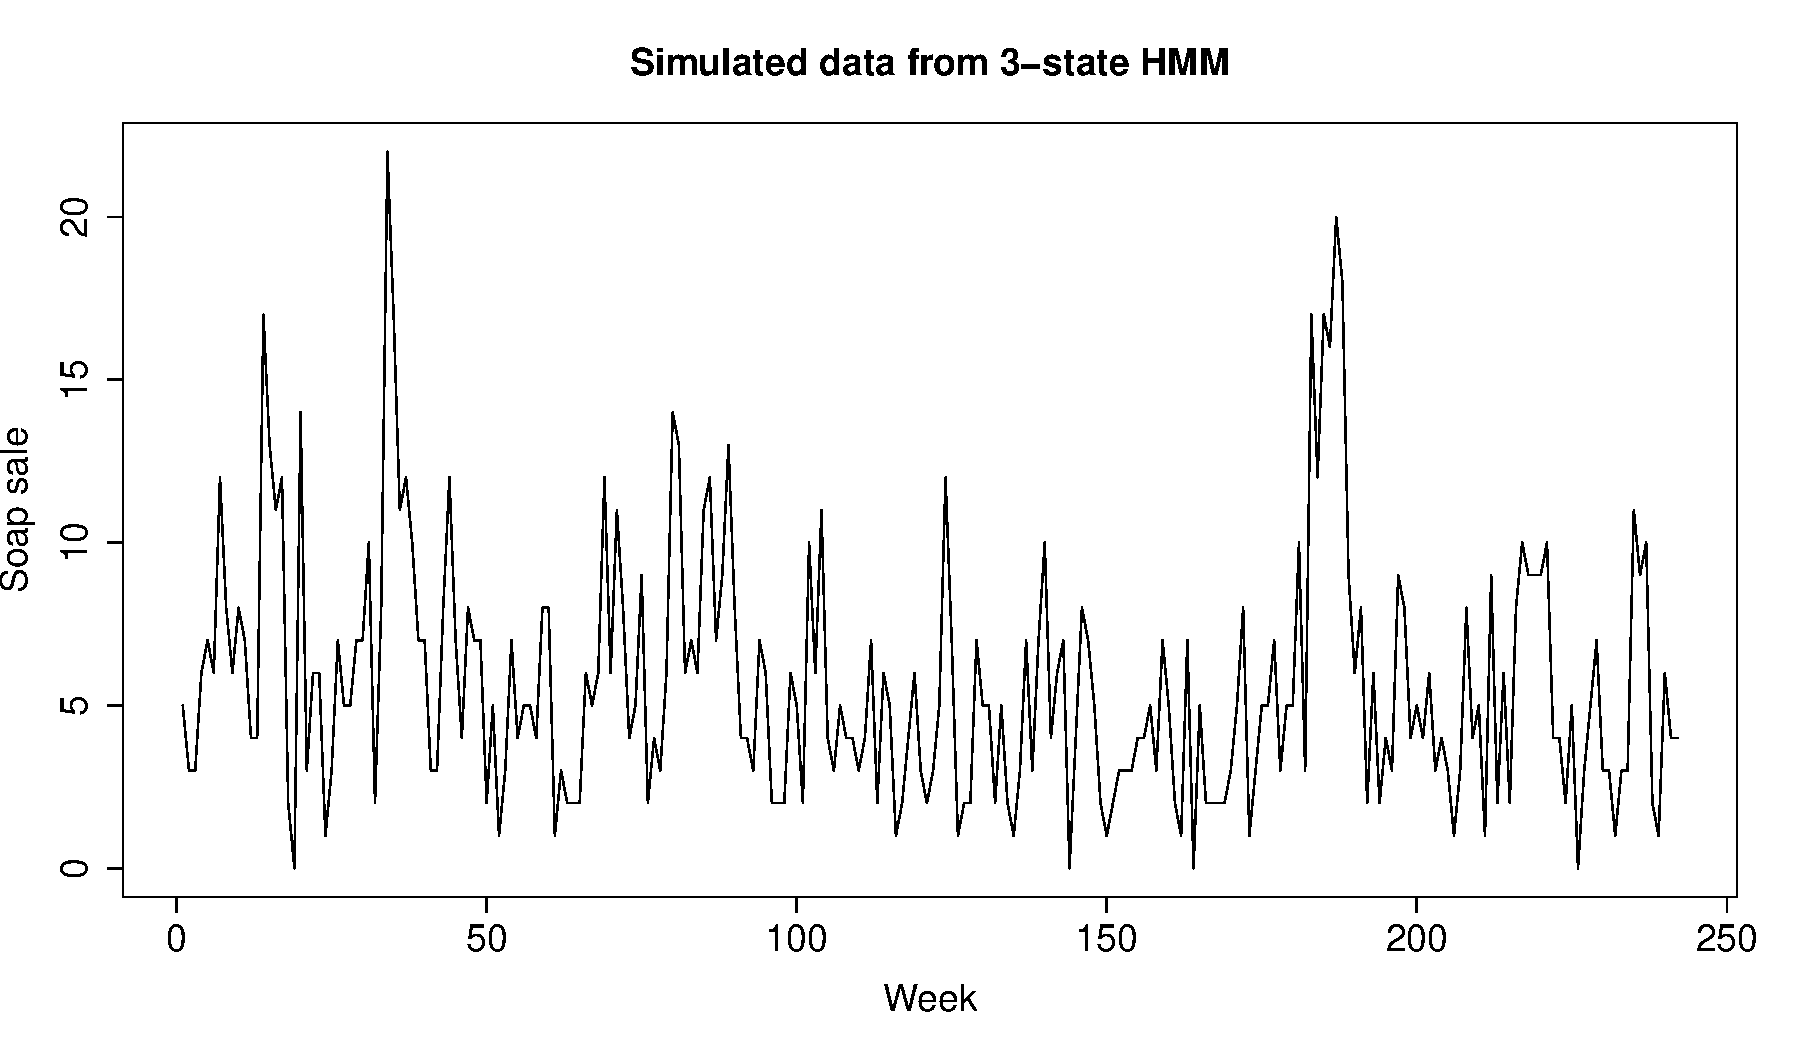
\includegraphics[width=260px]{../plots/3-state-sim-1.pdf}}
    \only<2>{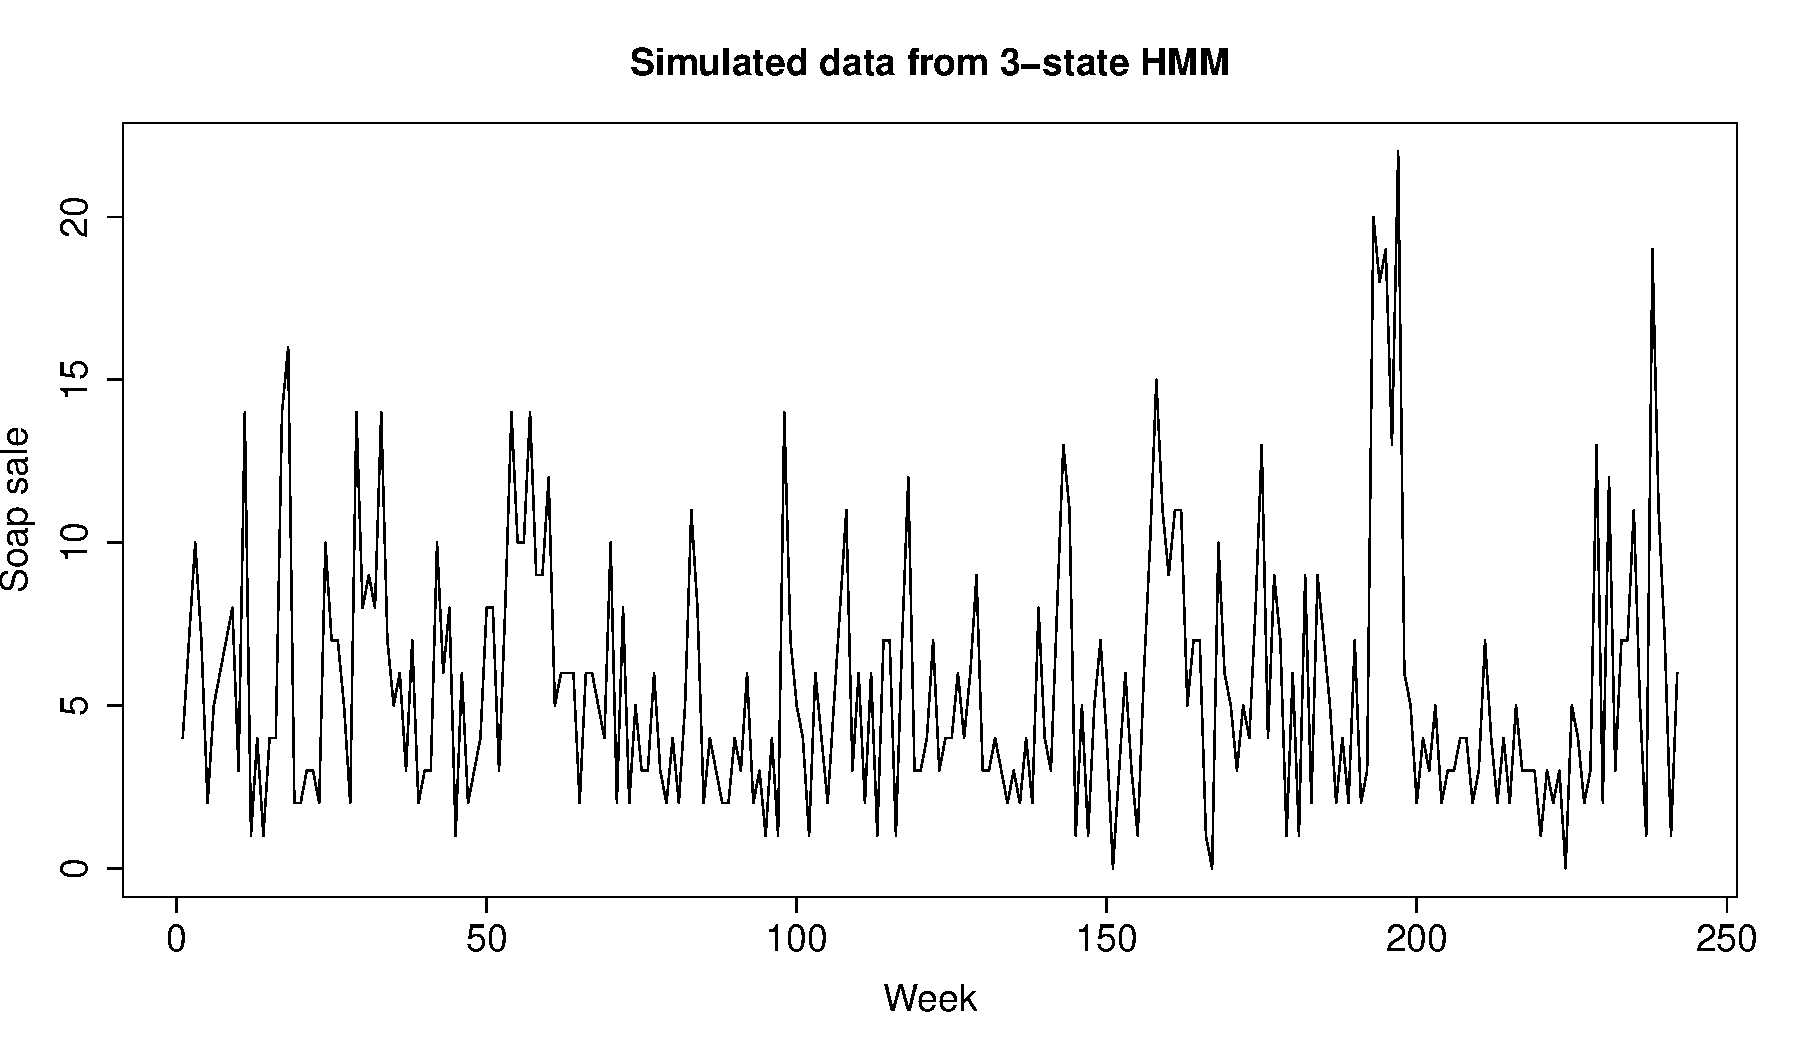
\includegraphics[width=260px]{../plots/3-state-sim-2.pdf}}
    \only<3>{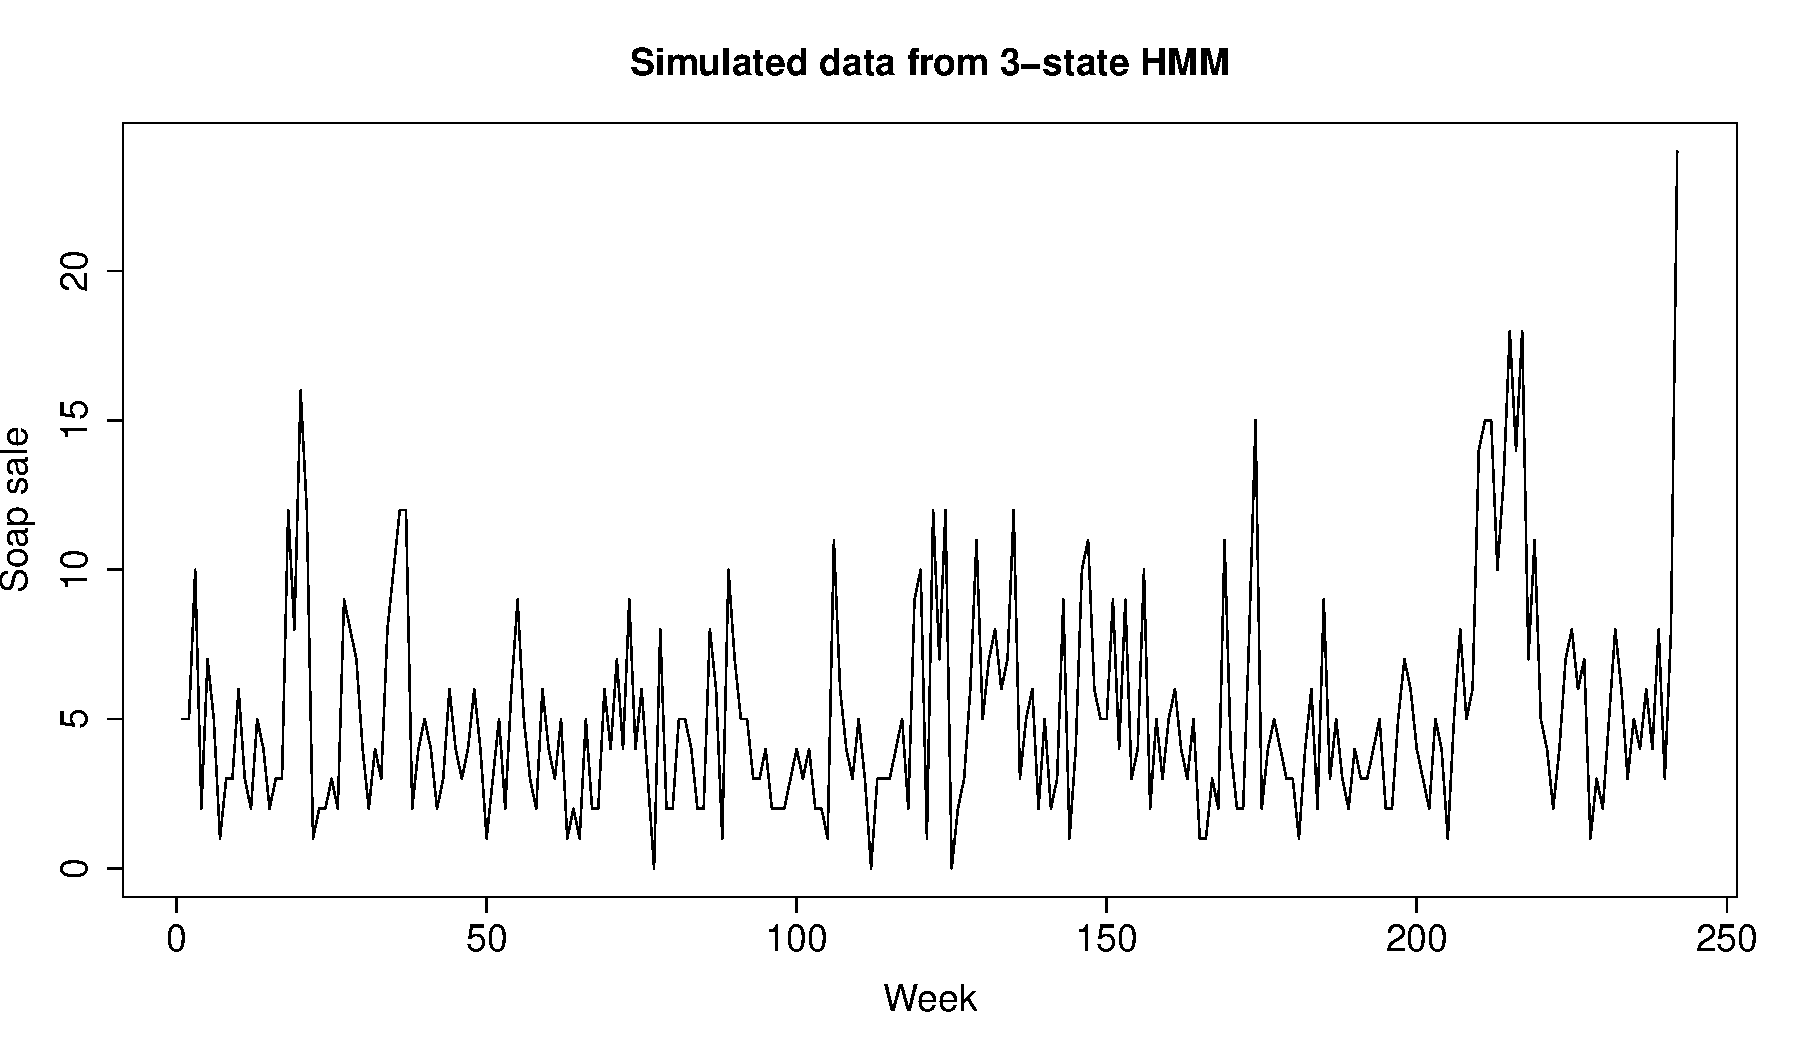
\includegraphics[width=260px]{../plots/3-state-sim-3.pdf}}
    \only<4>{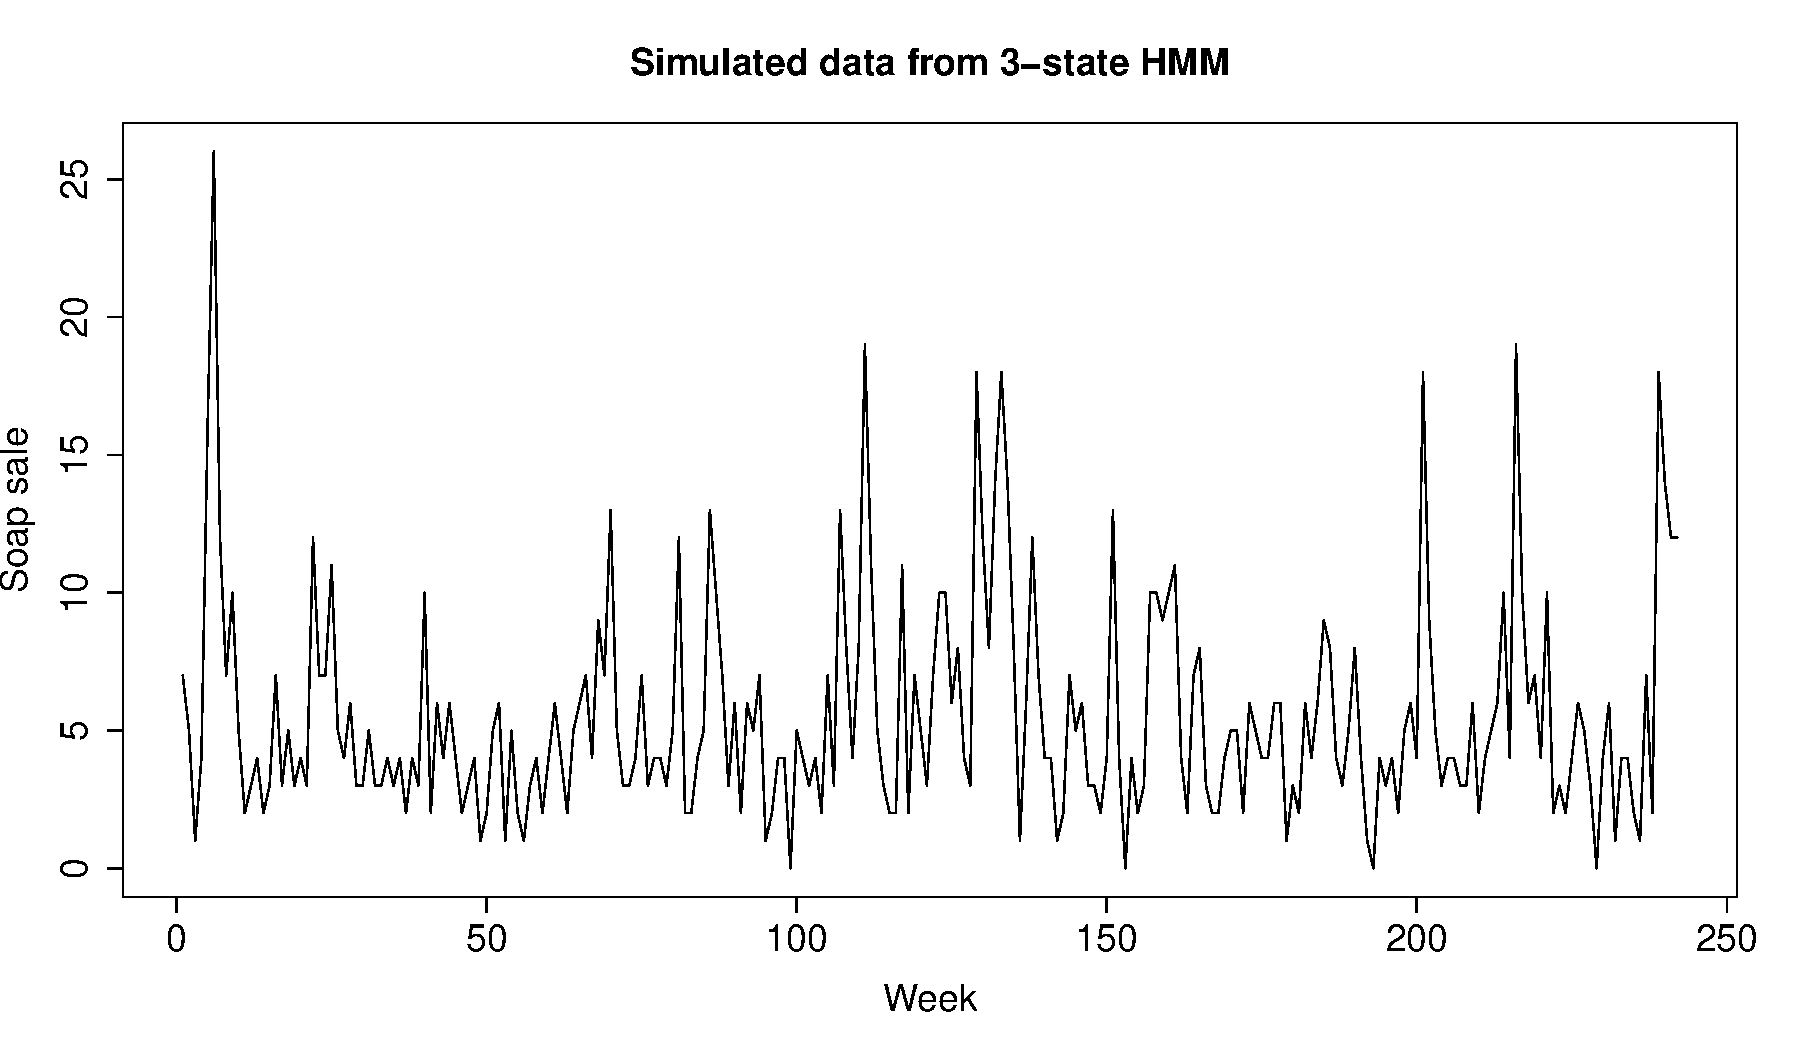
\includegraphics[width=260px]{../plots/3-state-sim-4.pdf}}
    \only<5>{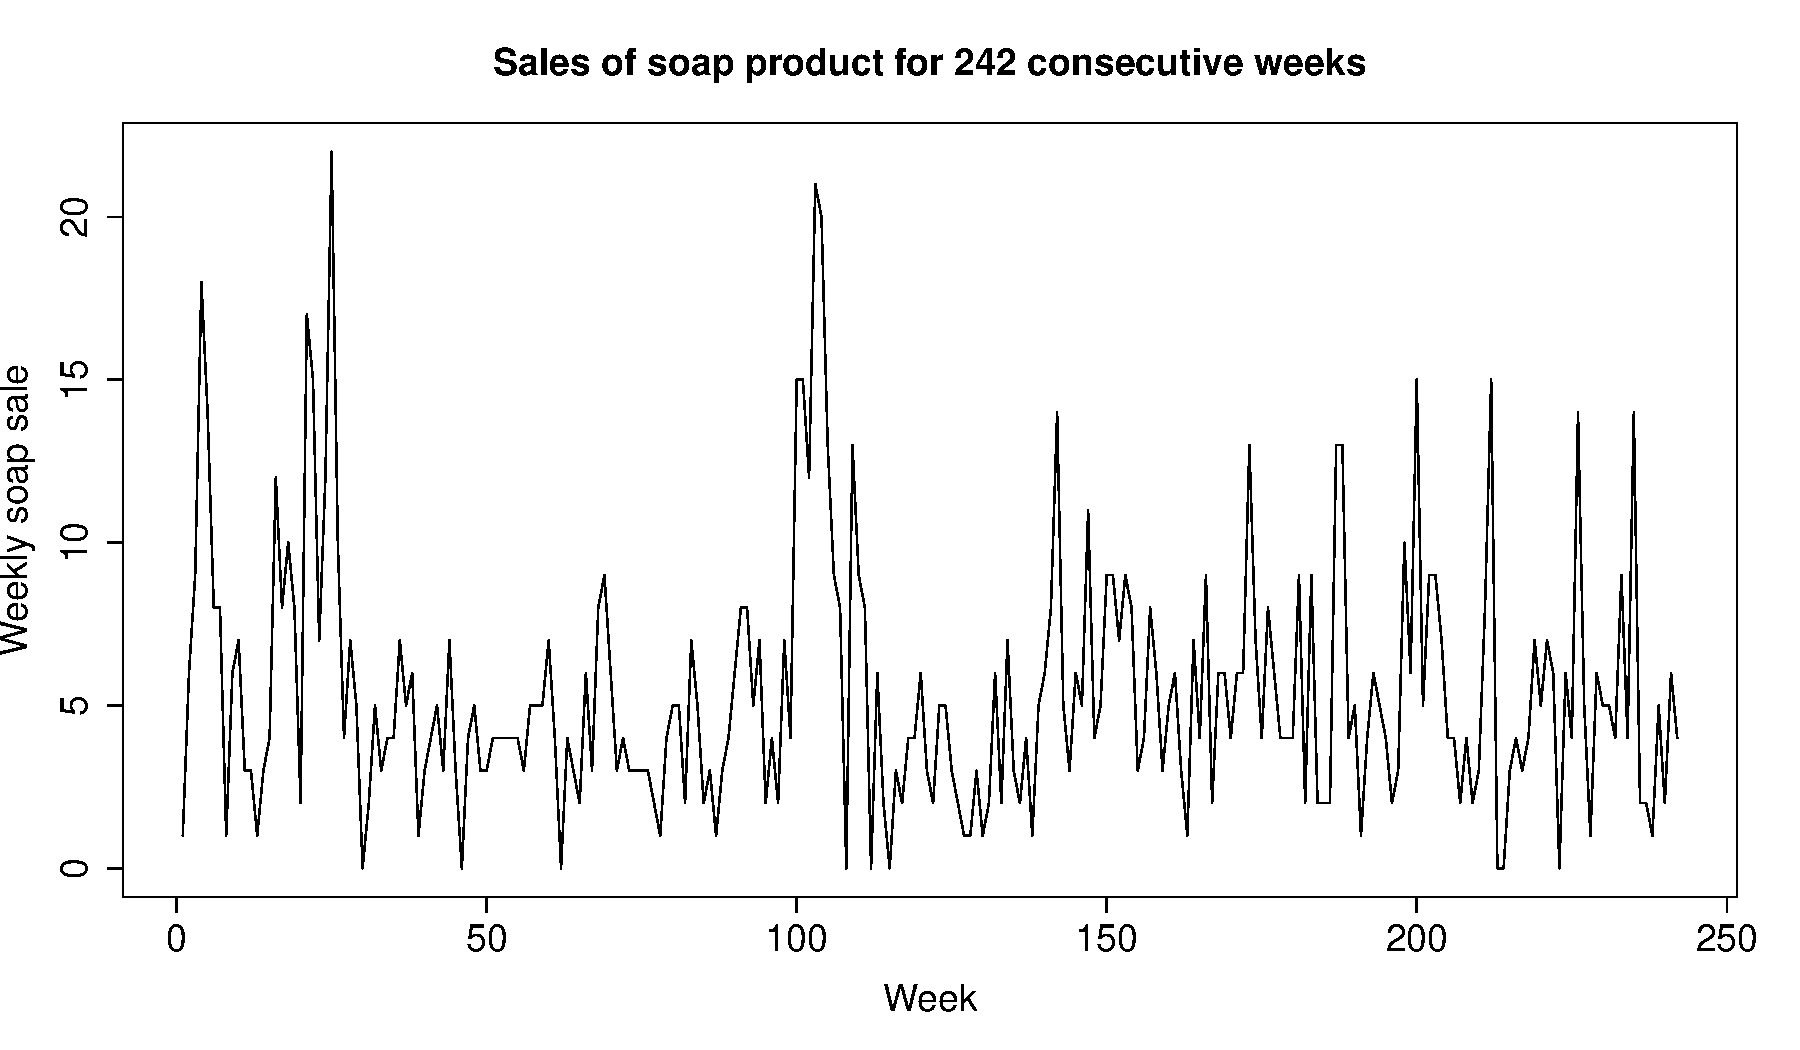
\includegraphics[width=260px]{../plots/sales-series.pdf}}
    \end{figure}
\end{frame}

\begin{frame}{Direct maximmization vs EM}
    Comparing direct maximization (DM) vs EM was the main focus of the exercise
    \begin{itemize}
        \item Similar parameter estimates was obtained
        \item The likelihood for the EM algorithm was a bit higher as expected, since stationarity was assumed for DM but not for EM
        \item In principle EM solves a harder problem, but $\myvec{\delta}_0$ can be shown to be a unit vector, and $m$ different simpler maximizations can be performed.
        \item For some initial parameter values the \myverb{nlm} function gave \myverb{NA} values when using the DM method.
    \end{itemize}
\end{frame}

\begin{frame}{Direct maximmization vs EM performance}
    \begin{itemize}
        \item In report it is concluded that no significant difference in performance is noticed. This was a qualitative remark.
        \item In section 4.4 in the course text book the DM method is mentioned to converge faster than EM.
        \item Let's try to time the performance of the two methods using the \myverb{system.time} function in R.
    \end{itemize}
\end{frame}

\begin{frame}{Comparing performance of Direct Maximization vs EM}
    Runtime for the two algorithms. Each run is done with 9 different initial values.
    \begin{columns}[t]
        \begin{column}{5cm}
            Direct maximization
            \lstinputlisting{../results/timing-2-ml}
            \lstinputlisting{../results/timing-3-ml}
            \lstinputlisting{../results/timing-4-ml}
        \end{column}
        \begin{column}{5cm}
            EM algorithm
            \lstinputlisting{../results/timing-2-em}
            \lstinputlisting{../results/timing-3-em}
            \lstinputlisting{../results/timing-4-em}
        \end{column}
    \end{columns}
\end{frame}

\begin{frame}{Conclusion?}
    \begin{itemize}
        \item Large difference in performance for 3-state and especially 4-state models.
        \item EM is seen to perform much better than DM for 4-states.
        \item Opposite of the remarks in section 4.4 in Zucchini 09
    \end{itemize}
\end{frame}


\begin{frame}{Questions}
    Time for some questions...
\end{frame}


\end{document}
